\documentclass[conference]{IEEEtran}

\usepackage[spanish]{babel}
\usepackage{amsmath,amssymb,amsfonts,amsthm}
\usepackage{graphicx}
\usepackage[utf8]{inputenc} % Caracteres en Español (Acentos, ñs)
\usepackage{url} % ACENTOS
\usepackage{hyperref} % Referencias
\usepackage{subfig}
\usepackage{lipsum}
\usepackage{balance} 
\usepackage{etoolbox}
\makeatletter
\patchcmd{\frontmatter@RRAP@format}{(}{}{}{}
\patchcmd{\frontmatter@RRAP@format}{)}{}{}{}
\makeatother	

\usepackage[backend=bibtex,sorting=none]{biblatex}
\setcounter{biburllcpenalty}{7000}
\setcounter{biburlucpenalty}{8000}
\addbibresource{references.bib}

% fecha
\usepackage{datetime}
\newdateformat{specialdate}{
    \twodigit{\THEDAY}-\twodigit{\THEMONTH}-\THEYEAR
}
\date{\specialdate\today}

% la sentencia \burl en las citas... 
\usepackage[hyphenbreaks]{breakurl}
\renewcommand\spanishtablename{Tabla}
\renewcommand\spanishfigurename{Figura}


\begin{document}
% Definitions
\newcommand{\breite}{0.9} %  for twocolumn
\newcommand{\RelacionFiguradoscolumnas}{0.9}
\newcommand{\RelacionFiguradoscolumnasPuntoCinco}{0.45}

%Title of paper
\title{Reporte de Laboratorio 2 \\ Subtitulado en Tiempo Real}

% Trabajo Individual
\author{
    \IEEEauthorblockN{
        Ricardo Emmanuel Uriegas Ibarra\IEEEauthorrefmark{1}
        }
    % En caso de trabajos en equipo, poner a todos los autores 
    % en estricto ORDEN ALFABETICO
    %\author{\IEEEauthorblockN{Michael Shell\IEEEauthorrefmark{1},
    %Homer Simpson\IEEEauthorrefmark{1}}
    \IEEEauthorblockA{
        \IEEEauthorrefmark{1}Ingeniería en Tecnologías de la Información\\
        Universidad Politécnica de Victoria
    }
}

\maketitle

%%%%%%%%%%%%%%%%%%%%%%%%%%%%%%%%%%%%%%%%%%%%%%%%%%%%%%%%%%%%%%%%%%%%%%%
\begin{abstract} 

\end{abstract}

%%%%%%%%%%%%%%%%%%%%%%%%%%%%%%%%%%%%%%%%%%%%%%%%%%%%%%%%%%%%%%%%%%%%%%%
\section{Introducción}
Existe una gran diversidad de públicos alrededor del mundo, uno de estos públicos son las personas con discapacidad auditiva, aproximadamente un 5\% de la población mundial tiene discapacidad auditiva, lo que significa que aproximadamente 466 millones de personas en el mundo tienen esta problemática. \cite{OMS}

En distintas industrias se han desarrollado tecnologías para ayudar a las personas con esta discapacidad, una de estas tecnologías es el subtitulado en tiempo real, el cual consiste en mostrar en tiempo real lo que se esta diciendo en algún tipo de contenido audiovisual; esto ayuda a estas personas a poder seguir disfrutando de este tipo de contenido sin necesidad de tener que contar con un interprete de lenguaje de señas.

%%%%%%%%%%%%%%%%%%%%%%%%%%%%%%%%%%%%%%%%%%%%%%%%%%%%%%%%%%%%%%%%%%%%%%%
\section{Desarrollo Experimental}
En este proyecto se desarrollo un sistema de subtitulado en tiempo real en PyQt6. El programa muestra en tiempo real los subtítulos que se obtienen del micrófono junto al video dado por la cámara. De igual manera permite guardar un video con los subtítulos en formato \textit{.mp4}, un video limpio sin los subtítulos en formato \textit{.mp4} y un archivo \textit{.srt} con los subtítulos generados por el programa (con un leve retraso para encajar de mejor manera con el audio del video). El proyecto se desarrollo en Python con interfaz Qt6; utilizando la librería de OpenCV para el procesamiento de video y la librería de SpeechRecognition para el reconocimiento de voz (librerías vistas en clases anteriores), entre otras librerías como PyAudio, Numpy, etc.

\subsection{Procesamiento de audio}
Para la recolección del audio se utilizó la librería PyAudio. El flujo de trabajo inicia con la configuración del micrófono, seguida de la captura de fragmentos de audio. Posteriormente, estos fragmentos se procesan en segundo plano, y la librería SpeechRecognition se encarga de convertirlos en texto (subtítulos) en tiempo real.

\subsection{Procesamiento de video}
El video es capturado por la cámara del dispositivo mediante la librería OpenCV, el video se muestra en tiempo real en un widget de la interfaz gráfica junto a los subtítulos generados por el procesamiento de audio. Para mostrar los subtitulos junto al video se utiliza la librería Pillow que permite la superposición de texto en una imagen, la razón de esta decision sobre la librería OpenCV es que Pillow permite acentos y caracteres especiales en el texto, mientras que OpenCV pareciera no soportar estos caracteres.

\subsection{Subtitulado en tiempo real}
Aquí es donde el proceso de audio junto al procesamiento de video se unen. Esta combinación consiste en mostrar en tiempo real los subtítulos que se obtienen del micrófono, mientras se muestra el video dado por la cámara.

Para lograr esta combinación en el código se utilizo un hilo para el procesamiento de audio y otro hilo para el procesamiento de video. De esta manera se logra que ambos procesos se ejecuten de manera simultanea. 

\subsection{Guardado de video con subtítulos}
El programa permite guardar el video con subtítulos, mientras al mismo tiempo generara 2 archivos; un archivo de video limpio (.mp4) y un archivo de subtítulos (.srt) que permite visualizar los subtítulos en cualquier reproductor de video de forma mas sincronizada, puesto que el principal guardado posee un retraso entre el audio y los subtítulos, generado por la generación de estos en tiempo real.

Es importante reconocer que al tratarse de 2 hilos independientes para el procesamiento de audio y video, se generan retrasos en la sincronización de los subtítulos con el audio del video, por lo que a prueba y error se determino un retraso de 1.6 segundos del video limpio en conjunto a los subtítulos (archivo .srt) para lograr una sincronización mejorada; de igual manera al tratarse de un archivo .srt, se puede ajustar el tiempo de inicio y fin de cada subtitulo para lograr una sincronización perfecta en caso de que el programa no logre sincronizar correctamente algunas partes del video.


%%%%%%%%%%%%%%%%%%%%%%%%%%%%%%%%%%%%%%%%%%%%%%%%%%%%%%%%%%%%%%%%%%%%%%%
\section{Resultados}
La interfaz del programa es relativamente simple, y con funcionalidades mínimas. Primeramente tenemos que haber leído el README del proyecto donde se mencionan los requerimientos del programa, su instalación, y mas importante aun; como usar el programa. El programa tiene 2 modos de uso, el modo de grabación y el modo de visualización en tiempo real. Para comenzar el modo grabación o concluirla, el usuario debe presionar la letra 'r' en el teclado. De igual maneta para concluir la ejecución del programa el usuario debe presionar la letra 'q' en el teclado.

En la figura \ref{fig:default-UI} se muestra la interfaz gráfica del programa al ejecutarse. Posteriormente se muestra como es que la interfaz se mira al presionar la letra 'r', indicando que la grabación se encuentra en proceso \ref{fig:rec-UI}. Consecuentemente se muestra la ventana de guardado de archivos \ref{fig:save-window} después de presionar nuevamente la letra 'r' donde el usuario asigna un nombre a los archivos generados por el programa, y por ultimo se observan los archivos generados por el mismo \ref{fig:generated-images} (en este caso se mantuvo el nombre por defecto de los archivos, por lo tenemos 3 archivos; un video con subtítulos, un video limpio y un archivo .srt con los subtítulos generados por el programa).

% default-UI.png
\begin{figure}[ht]
    \centering
    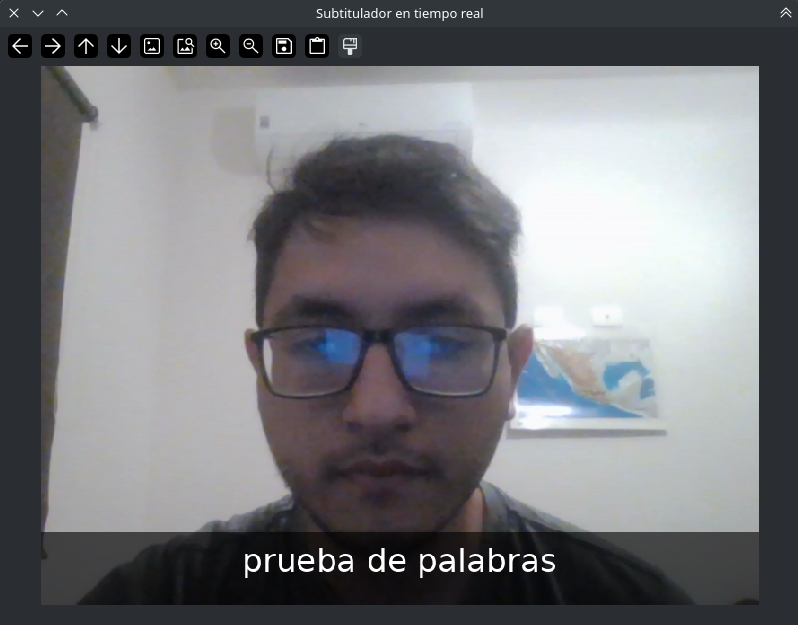
\includegraphics[width=\columnwidth]{images/default-UI.png}
    \caption{Interfaz gráfica del programa al ejecutarse.}
    \label{fig:default-UI}
\end{figure}

% generated-images.png
\begin{figure}[ht]
    \centering
    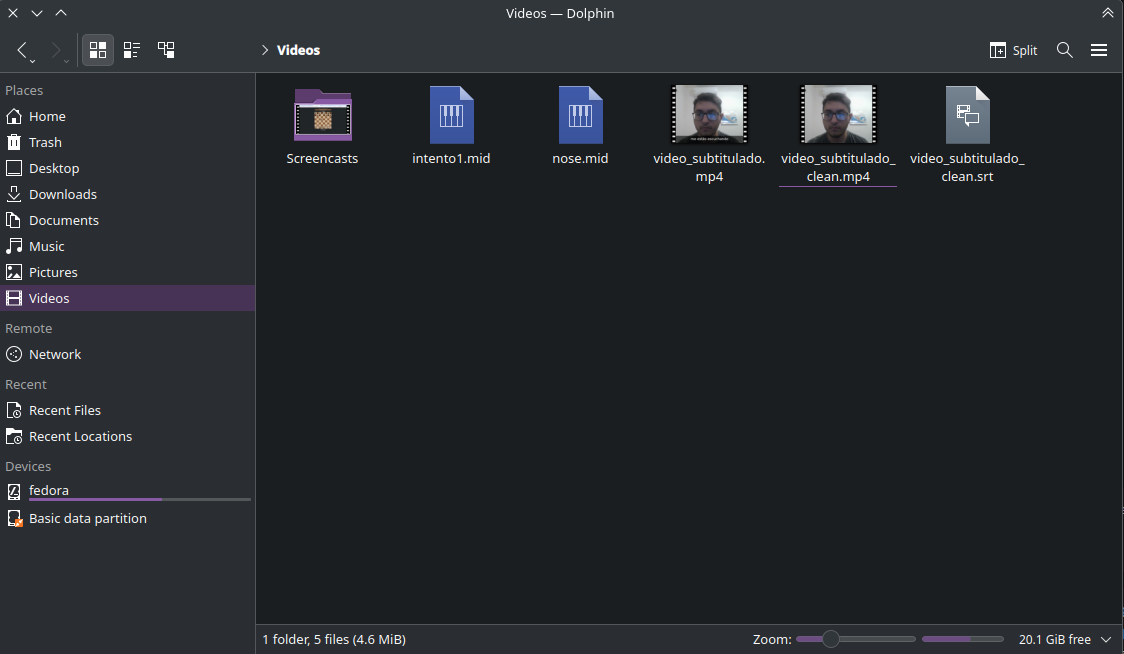
\includegraphics[width=\columnwidth]{images/generated-images.png}
    \caption{Ejemplo de los archivos generados por el programa al guardar un video.}
    \label{fig:generated-images}
\end{figure}

% rec-UI.png
\begin{figure}[ht]
    \centering
    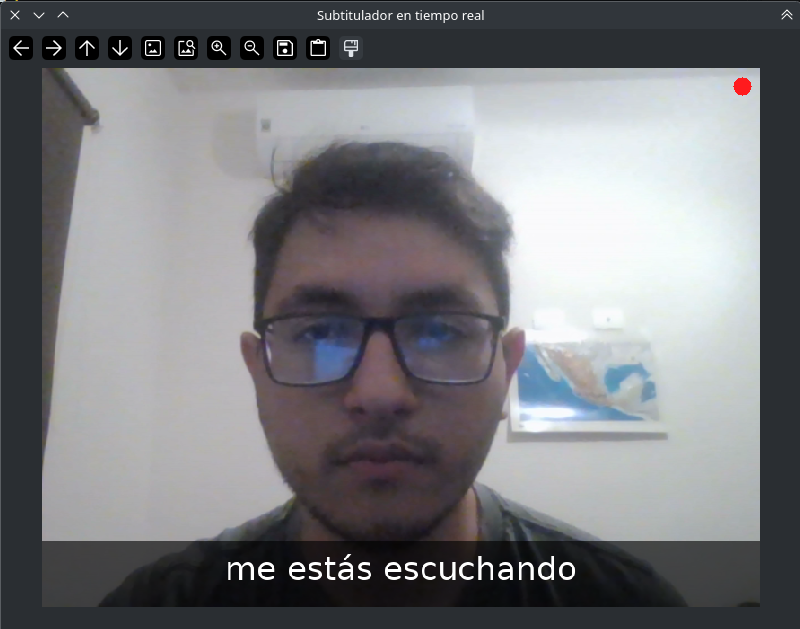
\includegraphics[width=\columnwidth]{images/rec-UI.png}
    \caption{Interfaz gráfica del programa al comenzar la grabación.}
    \label{fig:rec-UI}
\end{figure}

% save-window.png
\begin{figure}[ht]
    \centering
    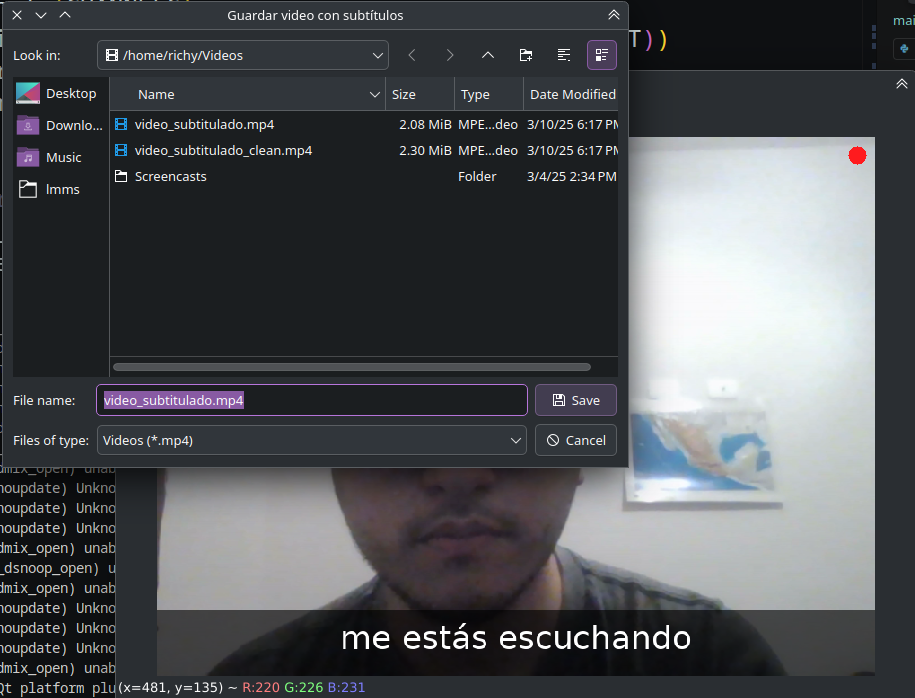
\includegraphics[width=\columnwidth]{images/save-window.png}
    \caption{Ventana de guardado de archivos generados por el programa.}
    \label{fig:save-window}
\end{figure}

%%%%%%%%%%%%%%%%%%%%%%%%%%%%%%%%%%%%%%%%%%%%%%%%%%%%%%%%%%%%%%%%%%%%%%%
\section{Conclusión}


%%%%%%%%%%%%%%%%%%%%%%%%%%%%%%%%%%%%%%%%%%%%%%%%%%%%%%%%%%%%%%%%%%%%%%%
\nocite{calcularRangos}
\addcontentsline{toc}{section}{Referencias} 
\printbibliography
%\balance

\end{document}